\graphicspath{{images/act_1.1/}}
\subsection{Generate sinusoidal reference}
\label{subsec:generate_sinusoidal_reference}
The objective of this activity is to generate a sinusoidal reference trajectory on the $x$-axis for $4$ seconds and then change to a constant reference trajectory. Likewise, the reference trajectory should start in position $p_0=\begin{bmatrix}  0.5765 &   0.1915 &   0.3637 \end{bmatrix}$ m. For this purpose, Algorithm \ref{lst:sine_reference_generator} describes a function to generate a trajectory that change from sinusoidal to constant reference and consider initial end-effector position. Finally, Figure \ref{fig:act_1.1_sin_reference} shows the sinusoidal reference trajectories that robot end-effector will track in next activities. \vspace{.5cm}

\begin{lstlisting}[language=Python,caption=Function to generate a sinusoidal reference trajectory for some seconds and then change to a constant reference trajectory., label={lst:sine_reference_generator}]
def sinusoidal_reference_generator(q0, a, f, t_change, t):
    """
    @info: generates a sine signal.

    @inputs: 
    ------
        - q0: initial joint/cartesian position   [or rad or m]
        - a: amplitude [rad]
        - f: frecuency [hz]
        - t_change: time to make the change  [sec]
        - t: simulation time [sec]
    @outputs:
    -------
        - q, dq, ddq: joint/carteisan position, velocity and acceleration
    """
    w = 2*np.pi*f               # [rad/s]
    if t<=t_change:
        q = q0 + a*np.sin(w*t)      # [rad]
        dq = a*w*np.cos(w*t)        # [rad/s]
        ddq = -a*w*w*np.sin(w*t)    # [rad/s^2]
    else:
        q = q0 + a*np.sin(w*t_change)   # [rad]
        dq = 0                          # [rad/s]
        ddq = 0                         # [rad/s^2]
    return q, dq, ddq
\end{lstlisting}

\vspace*{0cm}
\begin{figure}
	\centering
	\subfloat[]{
	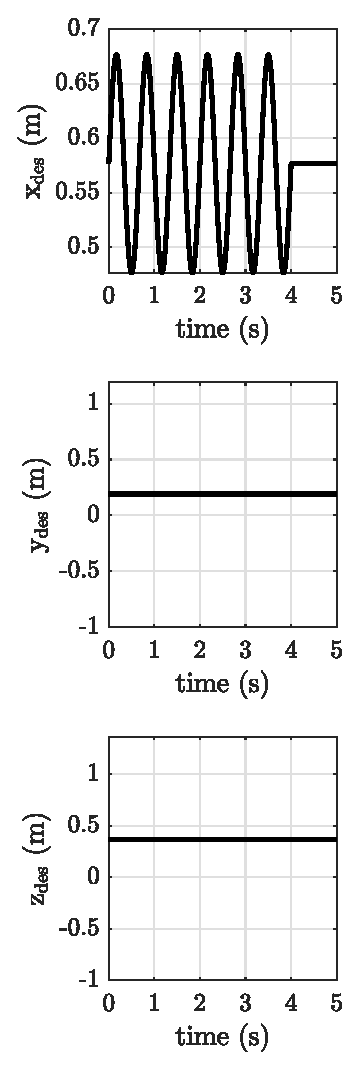
\includegraphics{ee_position.eps}
	%\caption{Reference position for the robot end-effector with Algorithm \ref{lst:sine_reference_generator}.}
	%\label{fig:act_1.1_ee_position}
	}
	\hfill
	\subfloat[]{
	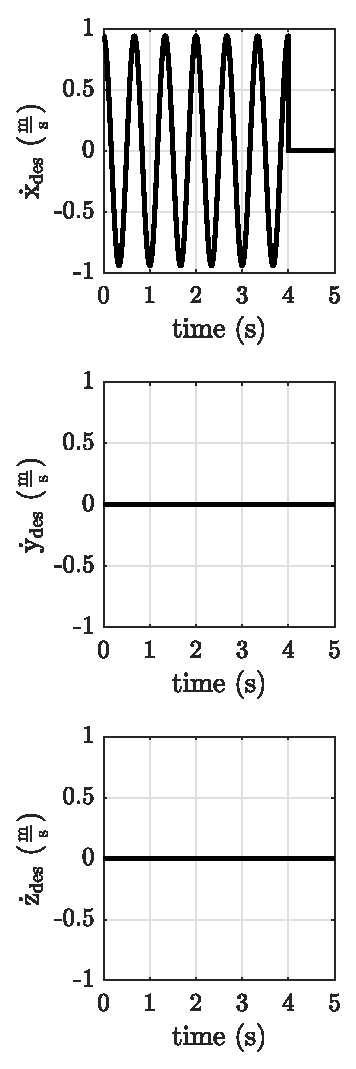
\includegraphics{ee_velocity.eps}
	%\caption{Reference velocity for the robot end-effector with Algorithm \ref{lst:sine_reference_generator}.}
	%\label{fig:act_1.1_ee_velocity}	
	}	
	\hfill
	\subfloat[]{
	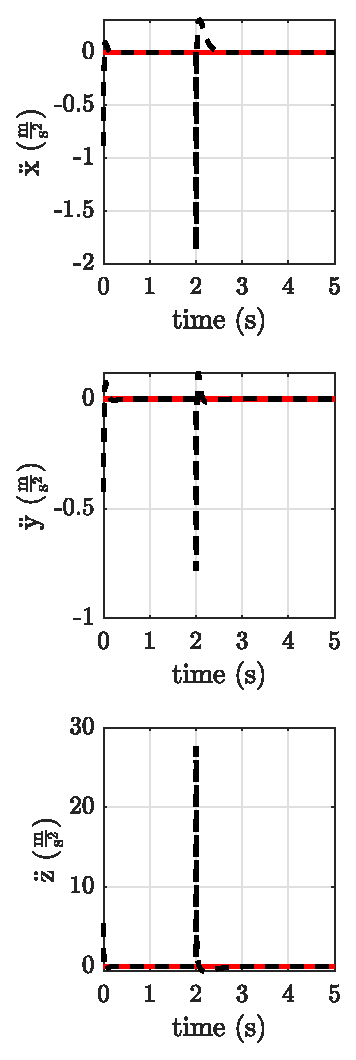
\includegraphics{ee_acceleration.eps}
	%\caption{Reference velocity for the robot end-effector with Algorithm \ref{lst:sine_reference_generator}.}
	%\label{fig:act_1.1_ee_acceleration}	
	}		
	\caption{Cartesian reference trajectories for the robot end-effector with Algorithm~\ref{lst:sine_reference_generator}: (a) position, (b) velocity and (c) acceleration.}
	\label{fig:act_1.1_sin_reference}
\end{figure}
